% chktex-file 2
% chktex-file 8
% chktex-file 11
% chktex-file 24
% chktex-file 26
\chapter{Introduzione}
\label{cap:introduzione}
%\begin{figure}[h!]
%    \centering
%    \includegraphics[width=1\columnwidth]{img/quantum_entanglement.png}
%    \caption{Lorem}
%    \label{fig:entanglement}
%\end{figure}
%
%Introduzione al contesto applicativo.
%
%Lorem Figure \ref{fig:entanglement}
%
%Esempio di utilizzo di un termine nel glossario \gls{api}.
%
%Esempio di citazione in linea
%\cite{site:agile-manifesto}.
%
%Esempio di citazione nel pie' di pagina
%citazione\footcite{womak:lean-thinking}
%
%Termine di glossario \gls{apig}
%
%\lipsum[1-2]
\emph{In questo capitolo andremo ad analizzare l'azienda ospitante dello stage descrivendo la sua organizzazione e le principali attività svolte. Verrà poi presentata l'offerta di stage proposta dall'azienda, con particolare attenzione agli obiettivi del progetto e alle tecnologie coinvolte. Infine, verrà fornita una panoramica sull'organizzazione del testo.}

\section{Profilo aziendale}
\myCompany (logo in figura \ref{fig:logo_sanmarco})  è un'azienda italiana specializzata nello sviluppo software e nella consulenza informatica. Da oltre quarant'anni, \myCompany si dedica alla riorganizzazione dei processi aziendali in diversi settori, progettando e implementando soluzioni digitali integrate. Con un forte orientamento verso l'innovazione, l'azienda si prefigge di agevolare la trasformazione digitale dei propri clienti, contribuendo al loro progresso.

\begin{figure}[h!]
    \centering
    
\includegraphics[width=0.6\columnwidth]{img/logo_sanmarco_informatica.png}
    \caption{Logo di Sanmarco Informatica}
    \label{fig:logo_sanmarco}
\end{figure}

L'innovazione rappresenta il pilastro fondamentale di \myCompany. L'azienda si impegna a essere costantemente riconosciuta come altamente innovativa, investendo tra il 15\% e il 20\% del fatturato annuo in attività di Ricerca e Sviluppo. Questo investimento, unito alla capacità di cogliere idee e suggerimenti da clienti, dipendenti e collaboratori, alimenta lo sviluppo di nuovi prodotti e soluzioni. Particolare attenzione è riservata agli aspetti sociali e alla riduzione dell'impatto ambientale.

Oltre all'innovazione, \myCompany si distingue per l'eccellenza del servizio offerto ai propri clienti. Grazie alla competenza maturata dai suoi consulenti attraverso un'esperienza pluriennale, l'azienda è in grado di proporre miglioramenti decisivi per rendere i processi aziendali più efficaci ed efficienti.

L'impegno verso la sostenibilità ambientale è un altro elemento chiave per \myCompany. L'azienda ha intrapreso un percorso volto alla riduzione drastica delle proprie emissioni nocive, dimostrando un forte senso di responsabilità verso l'ambiente.

\myCompany conta oggi oltre 600 dipendenti e più di 2500 aziende clienti. La sede principale si trova presso Villa Romanelli a Grisignano di Zocco, in provincia di Vicenza, nelle vicinanze dei Centri di Ricerca e Sviluppo e del Centro per la Formazione di Vicenza. L'azienda dispone inoltre di filiali in Trentino-Alto Adige, Friuli-Venezia Giulia, Lombardia, Piemonte, Emilia-Romagna, Toscana, Campania e Puglia.

Maggiori informazioni sull'azienda sono disponibili sul sito web ufficiale\footnote{\url{https://www.sanmarcoinformatica.com/}}.


\subsection{\emph{Business Unit}}
L'azienda è organizzata in \emph{Business Unit} (figura \ref{fig:business_unit}), centri di competenza specifici e autonomi, ma in costante relazione tra loro. Ciascuna \emph{Business Unit} è specializzata in un settore particolare ed è composta da \emph{team} di sviluppo, consulenti e \emph{project manager}, che collaborano per garantire la massima qualità e la piena soddisfazione dei clienti. \myCompany dispone di 10 \emph{Business Unit} principali:

\begin{itemize}
    \item \textbf{\emph{Jgalileo}}: Si tratta della soluzione di \glsfirstoccur{\gls{erp}} che ha reso celebre \myCompany. \emph{Jgalileo} copre l'intero processo aziendale in modo integrato, permettendo di coordinare la filiera senza sprechi di tempo o risorse;
    \item \textbf{\emph{SMITech}}: Specializzata nelle soluzioni per la \glsfirstoccur{\gls{dataprotectiong}}, \emph{SMITech} offre servizi di \glsfirstoccur{\gls{cybersecurityg}},  gestione \glsfirstoccur{\gls{ibmpowerg}}, progetti di infrastruttura \glsfirstoccur{\gls{itg}}, e consulenza su \emph{privacy} e \glsfirstoccur{\gls{gdpr}}, migliorando la sicurezza e l'efficienza informatica delle aziende;
    \item \textbf{\emph{NextBI}}: Questa \emph{Business Unit} si occupa di \glsfirstoccur{\gls{businessintelligenceg}}, \glsfirstoccur{\gls{performancemanagementg}} e \glsfirstoccur{\gls{customerintelligenceg}}. La piattaforma proprietaria di \emph{NextBI} consente di gestire \emph{budget}, controllo, analisi, simulazioni strategiche e di ottenere dati in tempo reale attraverso algoritmi avanzati;
    \item \textbf{\emph{ECM}}: Dedicata alla gestione della documentazione digitale, \emph{ECM (Enterprise Content Management)}
    fornisce strumenti per gestire l'intero ciclo di vita dei contenuti elettronici;
    \item \textbf{\emph{Discovery Quality}}: Specializzata nella gestione della \glsfirstoccur{\gls{governanceaziendaleg}}, del sistema della qualità e dei processi aziendali, \emph{Discovery Quality} coordina in modo proattivo e strutturato i diversi enti coinvolti, siano essi interni o esterni, e permette un monitoraggio continuo grazie a potenti strumenti di analisi;
    \item \textbf{\emph{Factory}}: Dedicata alla \glsfirstoccur{\gls{supplychaing}} e alle \glsfirstoccur{\gls{operationsg}} nella fabbrica del futuro, \emph{Factory} offre una serie di \emph{software} per ottimizzare la gestione della produzione, migliorare il livello di servizio ai clienti, ridurre i livelli di scorta di magazzino e massimizzare i profitti riducendo i costi. Tra gli strumenti offerti figurano il \emph{Manufacturing Execution System (JMES)}, l'\emph{Advanced Planning \& Scheduling (APS)} e il \emph{Supply Chain Collaboration (SCC)};
    \item \textbf{\emph{JPA}}: Questa \emph{Business Unit} è focalizzata sul \glsfirstoccur{\gls{bpm}}, fornendo \emph{software} per creare, gestire e automatizzare i processi aziendali. \emph{JPA} consente di integrare e gestire i flussi di lavoro tra diverse aree funzionali e sistemi, riducendo il margine di errore e migliorando l'efficienza operativa;
    \item \textbf{\emph{JPM}}: \emph{JPM} è il \emph{software} di \glsfirstoccur{\gls{projectmanagementg}} sviluppato per supportare le aziende nella gestione dei progetti, facilitando il raggiungimento degli obiettivi di \emph{business}. Offre strumenti avanzati per la pianificazione, l'esecuzione, il monitoraggio e il controllo dei progetti, accessibili da qualsiasi dispositivo;
    \item \textbf{\emph{4words}}: Specializzata in \emph{e-commerce}, sviluppo \emph{web} e \emph{app}, \emph{4words} offre servizi che vanno dalla realizzazione di siti \emph{web} alla creazione di applicazioni mobili, fino al posizionamento sui motori di ricerca, supportando le aziende nel loro \emph{marketing} digitale;
    \item \textbf{\emph{TCE}}: La \emph{Business Unit} \emph{TCE} è dedicata alla configurazione commerciale e tecnica, con un focus sull'ottimizzazione delle fasi di preventivazione e acquisizione degli ordini. Utilizzando la tecnologia \glsfirstoccur{\gls{cpq}}, \emph{TCE} permette alla forza vendite di configurare offerte personalizzate, automatizzando le complesse logiche commerciali e integrandosi con strumenti di disegno tecnico e renderizzazione 3D.
\end{itemize}

La \emph{Business Unit} di riferimento per lo \emph{stage} è \emph{ECM (Enterprise Content Management)}, con sede presso il Centro per la Formazione di Vicenza. Questo \emph{team} si occupa dello sviluppo e della manutenzione di servizi legati alla gestione dei documenti digitali, come ad esempio: la gestione documentale; \emph{Discovery XChange} inerente la conformità normativa sulla fatturazione elettronica; conservazione \glsfirstoccur{\gls{pec}} integrata con Aruba; \emph{Digifinder} (strumento per la ricerca di fatture elettroniche); \emph{Firmae} (servizio di firma digitale dei documenti), e molti altri.

\begin{figure}[h!]
    \centering
    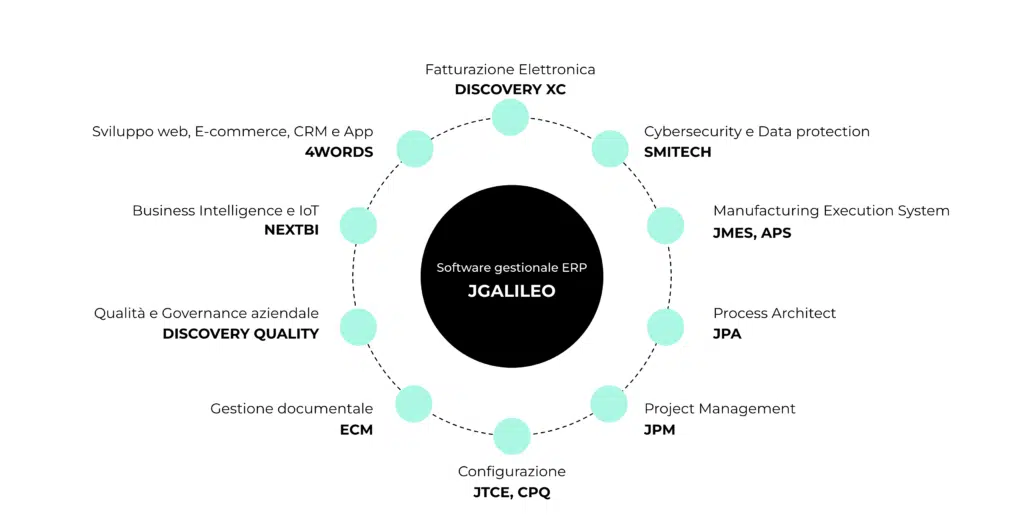
\includegraphics[width=0.8\columnwidth]{img/business_unit.png}
    \caption{Le \emph{Business Unit} di Sanmarco Informatica}
    \label{fig:business_unit}
\end{figure}

\subsection{Metodologia di sviluppo}
La metodologia di lavoro, indipendentemente dalla \emph{Business Unit}, è basata su un approccio \glsfirstoccur{\gls{agileg}} implementata con il framework \glsfirstoccur{\gls{scrumg}}. \gls{agileg} è un approccio alla gestione dei progetti che si fonda su principi di collaborazione, auto-organizzazione e flessibilità. \gls{scrumg} (figura \ref{fig:scrum}), in particolare, è un framework \gls{agileg} che facilita la gestione di progetti complessi, garantendo una maggiore flessibilità e adattabilità rispetto ai tradizionali metodi di sviluppo.

\begin{figure}[h!]
    \centering
    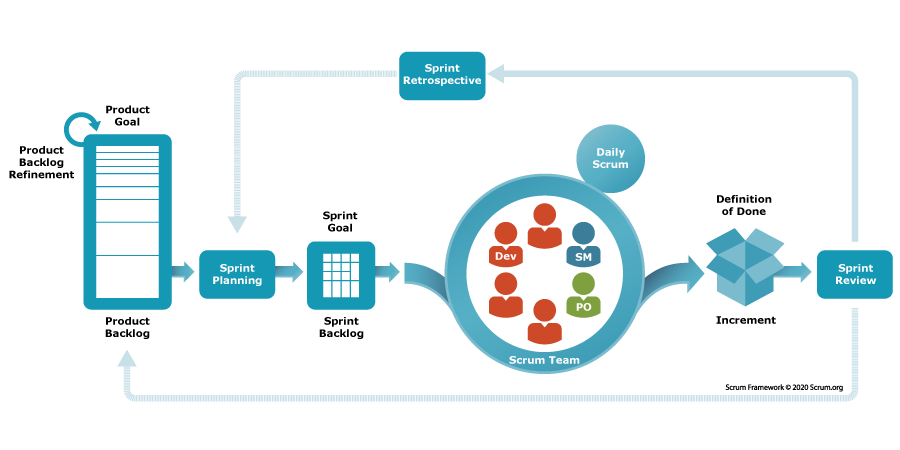
\includegraphics[width=0.9\columnwidth]{img/scrum.png}
    \caption{Il ciclo di sviluppo Scrum}
    \label{fig:scrum}
\end{figure}

\gls{scrumg} dunque si basa su tre principi fondamentali:
\begin{itemize}
    \item \textbf{Trasparenza}: Tutti i dettagli del progetto devono essere visibili a tutti i membri del \emph{team}, in modo che ciascuno possa avere una visione chiara e completa del lavoro svolto e da svolgere;
    \item \textbf{Ispezione}: Gli avanzamenti del progetto vengono ispezionati frequentemente per assicurarsi che il prodotto rimanga conforme ai requisiti e non si discosti dagli obiettivi;
    \item \textbf{Adattamento}: Se vengono rilevate discrepanze, il \emph{team} deve essere in grado di adattarsi rapidamente, modificando le parti non conformi del prodotto per ridurre al minimo lo scarto rispetto agli obiettivi stabiliti.
\end{itemize}

Il ciclo di sviluppo \gls{scrumg} è strutturato in \emph{sprint}, ovvero periodi di tempo relativamente brevi, solitamente di durata variabile tra una e quattro settimane, in cui vengono fissati determinati obiettivi e attività. Ogni \emph{sprint} inizia con un \emph{meeting} di pianificazione (\textit{Sprint Planning Meeting}), durante il quale il \emph{team} di sviluppo esamina il lavoro svolto nello \emph{sprint} precedente e definisce i nuovi obiettivi. Gli obiettivi fissati per uno \emph{sprint} non possono essere modificati durante la sua esecuzione. Al termine dello \emph{sprint}, il \emph{team} presenta al committente una versione funzionante del prodotto, che include i progressi realizzati.

Per ogni \emph{sprint}, i requisiti vengono estratti dal \textit{Product Backlog}, una lista di funzionalità e miglioramenti desiderati per il prodotto, e inseriti nello \textit{Sprint Backlog}, l'insieme delle attività da svolgere durante lo \emph{sprint}, dove vengono suddivisi in \emph{task} (o \emph{ticket}), ciascuno dei quali rappresenta un'unità di lavoro da completare in un tempo limitato.

Per garantire la fattibilità del prodotto e mantenere un'organizzazione ottimale, \gls{scrumg} prevede una serie di eventi regolari:

\begin{itemize}
    \item \textbf{\emph{Sprint Planning Meeting}}: All'inizio di ogni \emph{sprint}, il \emph{team} di sviluppo si riunisce per selezionare il lavoro da svolgere e definire il tempo necessario per ogni requisito del \textit{Product Backlog};
    \item \textbf{\emph{Daily Scrum}}: Durante lo \emph{sprint}, il \emph{team} si incontra quotidianamente per un breve \emph{meeting} di massimo 15 minuti, in cui si discute del lavoro svolto, di quello previsto per la giornata successiva e degli eventuali problemi riscontrati;
    \item \textbf{\emph{Sprint Review}}: Alla fine dello \emph{sprint}, il \emph{team} si riunisce con il committente per esaminare i cambiamenti nei requisiti, valutare il lavoro svolto e discutere delle problematiche riscontrate;
    \item \textbf{\emph{Sprint Retrospective}}: Dopo lo \emph{Sprint Review}, il \emph{team} si riunisce per discutere dei punti di forza e di debolezza dello \emph{sprint} appena concluso, con l'obiettivo di individuare le aree di miglioramento e di definire le azioni correttive da intraprendere per il prossimo \emph{sprint}.
\end{itemize}

Ogni \emph{team} Scrum è strutturato per essere indipendente, con l'obiettivo di ottimizzare i \emph{feedback} ricevuti dal committente. Il \emph{team} è generalmente composto da tre ruoli principali:

\begin{itemize}
    \item \textbf{\emph{Product Owner}}: La persona che commissiona il progetto, segue lo sviluppo del prodotto e ne definisce i requisiti;
    \item \textbf{\emph{Team} di sviluppo}: Il gruppo di professionisti che lavora alla realizzazione del prodotto;
    \item \textbf{\emph{Scrum Master}}: La figura responsabile di mantenere il \emph{team} di sviluppo focalizzato e motivato, proteggendolo da distrazioni e ponendo sfide che favoriscano il miglioramento continuo.
\end{itemize}

\section{L'offerta di \emph{stage}}
L'obiettivo principale dello \emph{stage} consiste nello sviluppo di un sistema avanzato per la catalogazione delle \gls{pec}, integrando tecnologie di \glsfirstoccur{\gls{ai}} al fine di migliorare l'efficienza e l'accuratezza del processo.

Gli obiettivi specifici del progetto proposto durante lo \emph{stage} possono essere riassunti come segue:

\begin{itemize}
    \item \textbf{Catalogazione automatica potenziata tramite \gls{ai}}: L'obiettivo è implementare modelli di \glsfirstoccur{\gls{machinelearningg}} capaci di analizzare il contenuto delle \gls{pecg} importate e classificarle automaticamente in base al contenuto. L'uso di tecnologie di \gls{ai} consentirà di rilevare informazioni quali mittente, destinatario, data e argomento, migliorando significativamente l'efficienza del processo di catalogazione.

    \item \textbf{Integrazione con un sistema di gestione documentale}: Le informazioni estratte dalle \gls{pecg} saranno integrate all'interno di un sistema di gestione documentale. Questo permetterà di persistere le \emph{e-mail} nel sistema, generando i metadati necessari a partire dalle informazioni estratte e collocandole nella categoria appropriata.

    \item \textbf{Adattamento e apprendimento continuo}: Saranno implementati algoritmi di \gls{ai} in grado di adattarsi e apprendere continuamente dai dati, migliorando le prestazioni del sistema nel tempo. Tale processo includerà l'ottimizzazione dei modelli di \gls{machinelearningg} in base all'esperienza acquisita e ai \emph{feedback} degli utenti.

    \item \textbf{Utilizzo dei servizi \emph{cloud} di AWS}: Il progetto prevede l'utilizzo dei servizi \emph{cloud} offerti da \glsfirstoccur{\gls{aws}} per l'addestramento del modello di \gls{machinelearningg} e per l'erogazione del servizio. L'infrastruttura necessaria sarà configurata direttamente sul \emph{cloud} di \gls{awsg}, garantendo così scalabilità ed efficienza.
\end{itemize}

Il progetto è stato proposto dall'azienda in occasione dell'evento \emph{Stage IT} 2024, organizzato dall'Università degli Studi di Padova e promosso da Confindustria Veneto Est. Tale evento, avente una cadenza annuale, ha come obiettivo quello di facilitare l'incontro tra studenti e aziende, offrendo la possibilità di svolgere uno \emph{stage} formativo con un particolare focus sul settore \gls{ictg}.


\section{Organizzazione del testo}

\begin{description}
    \item[{\hyperref[cap:descrizione-stage]{Il secondo capitolo}}] descrive lo \emph{stage}, l'organizzazione, gli obiettivi e le attività svolte.
    
    \item[{\hyperref[cap:tecnologie]{Il terzo capitolo}}] approfondisce le tecnologie utilizzate oltre che gli strumenti e le metodologie di lavoro.
    
    \item[{\hyperref[cap:progettazione-codifica]{Il quarto capitolo}}] descrive la progettazione e la codifica del sistema sviluppato durante lo \emph{stage}.
    
    \item[{\hyperref[cap:sviluppi-futuri]{Il quinto capitolo}}] descrive i possibili sviluppi futuri del progetto.
    
    \item[{\hyperref[cap:conclusioni]{Il sesto capitolo}}] illustra le conclusioni e le considerazioni finali sul lavoro svolto.
\end{description}